\documentclass[]{article}
\usepackage{amssymb,amsmath}
\usepackage{ifxetex,ifluatex}
\ifxetex
  \usepackage{fontspec,xltxtra,xunicode}
  \defaultfontfeatures{Mapping=tex-text,Scale=MatchLowercase}
\else
  \ifluatex
    \usepackage{fontspec}
    \defaultfontfeatures{Mapping=tex-text,Scale=MatchLowercase}
  \else
    \usepackage[utf8]{inputenc}
  \fi
\fi
\usepackage{ctable}
\usepackage{float} % provides the H option for float placement
\usepackage{graphicx}
% We will generate all images so they have a width \maxwidth. This means
% that they will get their normal width if they fit onto the page, but
% are scaled down if they would overflow the margins.
\makeatletter
\def\maxwidth{\ifdim\Gin@nat@width>\linewidth\linewidth
\else\Gin@nat@width\fi}
\makeatother
\let\Oldincludegraphics\includegraphics
\renewcommand{\includegraphics}[1]{\Oldincludegraphics[width=\maxwidth]{#1}}
\ifxetex
  \usepackage[setpagesize=false, % page size defined by xetex
              unicode=false, % unicode breaks when used with xetex
              xetex,
              colorlinks=true,
              linkcolor=blue]{hyperref}
\else
  \usepackage[unicode=true,
              colorlinks=true,
              linkcolor=blue]{hyperref}
\fi
\hypersetup{breaklinks=true, pdfborder={0 0 0}}
\setlength{\parindent}{0pt}
\setlength{\parskip}{6pt plus 2pt minus 1pt}
\setlength{\emergencystretch}{3em}  % prevent overfull lines
\setcounter{secnumdepth}{0}

\title{ANOVA Template}
\author{(Username not set) (E-mail address not set)}
\date{2011-04-26 20:25 CET}

\begin{document}
\maketitle

\subsection{Description}

An ANOVA report with table of descriptives, diagnostic tests and
ANOVA-specific statistics.

\subsection{Introduction}

\textbf{Analysis of Variance} or \textbf{ANOVA} is a statistical
procedure that tests equality of means for several samples. It was first
introduced in 1921. by famous English statistician Sir Ronald Aylmer
Fisher.

\subsection{Model Overview}

One-Way ANOVA was carried out, with \emph{Gender} as independent
variable, and \emph{Internet usage in leisure time (hours per day)} as a
response variable. Factor interaction was taken into account.

\subsection{Descriptives}

In order to get more insight on the model data, a table of frequencies
for ANOVA factors is displayed, as well as a table of descriptives.

\subsubsection{Frequency Table}

Below lies a frequency table for factors in ANOVA model. Note that the
missing values are removed from the summary.

\ctable[pos = H, center, botcap]{lllll}
{% notes
}
 & \textbf{Cumul.
N} & \textbf{Cumul. \%}
\ML
male & 410 & 60.9212 & 410 & 60.9212
\\\noalign{\medskip}
female & 263 & 39.0788 & 673 & 100
\\\noalign{\medskip}
Total & 673 & 100 & 673 & 100
\LL
}

\subsubsection{Descriptive Statistics}

The following table displays the descriptive statistics of ANOVA model.
Factor levels and/or their combinations lie on the left hand side, while
the corresponding statistics for response variable are given on the
right-hand side.

\ctable[pos = H, center, botcap]{lllllllll}
{% notes
}
{% rows
\FL
\textbf{fac} & \textbf{min(resp)} & \textbf{max(resp)} & \textbf{mean(resp)} & \textbf{SD(resp)} & \textbf{median(resp)} & \textbf{IQR(resp)} & \textbf{skewness(resp)} & \textbf{kurtosis(resp)}
\ML
male & 0 & 12 & 3.2699 & 1.9535 & 3 & 3 & 0.9479 & 4.0064
\\\noalign{\medskip}
female & 0 & 12 & 3.0643 & 2.3546 & 2 & 3 & 1.4064 & 4.9089
\\\noalign{\medskip}
 & 0 & 10 & 3.3824 & 2.5822 & 3 & 2 & 1.2197 & 3.8058
\LL
}

\subsection{Diagnostics}

Before we carry out ANOVA, we'd like to check some basic assumptions.
For those purposes, normality and homoscedascity tests are carried out
alongside several graphs that may help you with your decision on model's
main assumptions.

\subsubsection{Diagnostics}

\paragraph{Univariate Normality}

We will use \emph{Shapiro-Wilk}, \emph{Lilliefors} and
\emph{Anderson-Darling} tests to screen departures from normality in the
response variable (\emph{Internet usage in leisure time (hours per
day)}).

\ctable[pos = H, center, botcap]{lll}
{% notes
}
{% rows
\FL
 & \textbf{W} & \textbf{p}
\ML
shapiro.test & 0.9001 & 0
\\\noalign{\medskip}
lillie.test & 0.168 & 0
\\\noalign{\medskip}
ad.test & 18.753 & 0
\LL
}

As you can see, applied tests confirm departures from normality.

\paragraph{Homoscedascity}

In order to test homoscedascity, \emph{Bartlett} and
\emph{Fligner-Kileen} tests are applied.

\ctable[pos = H, center, botcap]{lll}
{% notes
}
{% rows
\FL
 & \textbf{H} & \textbf{p}
\ML
fligner.test & 0.4629 & 0.4963
\\\noalign{\medskip}
bartlett.test & 10.7698 & 0.001
\LL
}

When it comes to equality of variances, applied tests yield inconsistent
results. While \emph{Fligner-Kileen test} confirmed the hypotheses of
homoscedascity, \emph{Bartlett's test} rejected it.

\subsubsection{Diagnostic Plots}

Here you can see several diagnostic plots for ANOVA model:

\begin{itemize}
\item
  residuals against fitted values
\item
  scale-location plot of square root of residuals against fitted values
\item
  normal Q-Q plot
\item
  residuals against leverages
\end{itemize}
\begin{figure}[htbp]
\centering
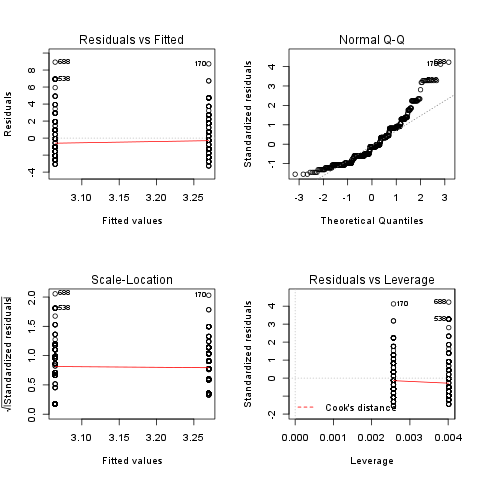
\includegraphics{1c63b6fad7856cf59a751b0f80339918.png}
\caption{}
\end{figure}

\subsection{ANOVA Summary}

\subsubsection{ANOVA Table}

\ctable[pos = H, center, botcap]{llllll}
{% notes
}
{% rows
\FL
 & \textbf{Df} & \textbf{Sum.Sq} & \textbf{Mean.Sq} & \textbf{F.value} & \textbf{Pr..F.}
\ML
gender & 1 & 6.4217 & 6.4217 & 1.4302 & 0.2322
\\\noalign{\medskip}
Residuals & 636 & 2855.63 & 4.49 &  & 
\LL
}

\emph{F-test} for \emph{Gender} is not statistically significant, which
implies that there is no Gender effect on response variable.

\subsection{Description}

An ANOVA report with table of descriptives, diagnostic tests and
ANOVA-specific statistics.

s

\subsection{Introduction}

\textbf{Analysis of Variance} or \textbf{ANOVA} is a statistical
procedure that tests equality of means for several samples. It was first
introduced in 1921. by famous English statistician Sir Ronald Aylmer
Fisher.

\subsection{Model Overview}

Two-Way ANOVA was carried out, with \emph{Gender} and \emph{Relationship
status} as independent variables, and \emph{Internet usage in leisure
time (hours per day)} as a response variable. Factor interaction was
taken into account.

\subsection{Descriptives}

In order to get more insight on the model data, a table of frequencies
for ANOVA factors is displayed, as well as a table of descriptives.

\subsubsection{Frequency Table}

Below lies a frequency table for factors in ANOVA model. Note that the
missing values are removed from the summary.

\ctable[pos = H, center, botcap]{llllll}
{% notes
}
 & \textbf{Cumul.
N} & \textbf{Cumul. \%}
\ML
male & in a relationship & 150 & 23.6967 & 150 & 23.6967
\\\noalign{\medskip}
female & in a relationship & 120 & 18.9573 & 270 & 42.654
\\\noalign{\medskip}
male & married & 33 & 5.2133 & 303 & 47.8673
\\\noalign{\medskip}
female & married & 29 & 4.5814 & 332 & 52.4487
\\\noalign{\medskip}
male & single & 204 & 32.2275 & 536 & 84.6761
\\\noalign{\medskip}
female & single & 97 & 15.3239 & 633 & 100
\\\noalign{\medskip}
Total & Total & 633 & 100 & 633 & 100
\LL
}

\subsubsection{Descriptive Statistics}

The following table displays the descriptive statistics of ANOVA model.
Factor levels and/or their combinations lie on the left hand side, while
the corresponding statistics for response variable are given on the
right-hand side.

\ctable[pos = H, center, botcap]{llllllllll}
{% notes
}
{% rows
\FL
\textbf{gender} & \textbf{partner} & \textbf{min(resp)} & \textbf{max(resp)} & \textbf{mean(resp)} & \textbf{SD(resp)} & \textbf{median(resp)} & \textbf{IQR(resp)} & \textbf{skewness(resp)} & \textbf{kurtosis(resp)}
\ML
male & in a
relationship & 0.5 & 12 & 3.0582 & 1.9692 & 2.5 & 2 & 1.3376 & 5.727
\\\noalign{\medskip}
male & married & 0 & 8 & 2.9848 & 2.029 & 3 & 2 & 0.9027 & 3.351
\\\noalign{\medskip}
male & single & 0 & 10 & 3.5027 & 1.9361 & 3 & 3 & 0.7636 & 3.1208
\\\noalign{\medskip}
male &  & 0.5 & 6.5 & 3.1304 & 1.7788 & 3 & 2.75 & 0.0719 & 1.9965
\\\noalign{\medskip}
female & in a
relationship & 0.5 & 10 & 3.0439 & 2.2158 & 3 & 3 & 1.4017 & 4.9165
\\\noalign{\medskip}
female & married & 0 & 10 & 2.4808 & 1.9671 & 2 & 1.75 & 2.1875 & 9.2864
\\\noalign{\medskip}
female & single & 0 & 12 & 3.3226 & 2.6791 & 3 & 3.5 & 1.2045 & 4.0139
\\\noalign{\medskip}
female &  & 0.5 & 6 & 2.6562 & 1.739 & 2 & 3 & 0.6914 & 2.4285
\\\noalign{\medskip}
 & in a
relationship & 0 & 8 & 3.3333 & 2.4398 & 3 & 2.5 & 0.7897 & 2.5973
\\\noalign{\medskip}
 & married & 2 & 7 & 3.8 & 1.9235 & 3 & 1 & 1.018 & 2.6519
\\\noalign{\medskip}
 & single & 0 & 10 & 3.5833 & 3.2039 & 3 & 1.5 & 1.279 & 3.4365
\\\noalign{\medskip}
 &  & 1 & 2 & 1.5 & 0.7071 & 1.5 & 0.5 & 0 & 1
\LL
}

\subsection{Diagnostics}

Before we carry out ANOVA, we'd like to check some basic assumptions.
For those purposes, normality and homoscedascity tests are carried out
alongside several graphs that may help you with your decision on model's
main assumptions.

\subsubsection{Diagnostics}

\paragraph{Univariate Normality}

We will use \emph{Shapiro-Wilk}, \emph{Lilliefors} and
\emph{Anderson-Darling} tests to screen departures from normality in the
response variable (\emph{Internet usage in leisure time (hours per
day)}).

\ctable[pos = H, center, botcap]{lll}
{% notes
}
{% rows
\FL
 & \textbf{W} & \textbf{p}
\ML
shapiro.test & 0.9001 & 0
\\\noalign{\medskip}
lillie.test & 0.168 & 0
\\\noalign{\medskip}
ad.test & 18.753 & 0
\LL
}

As you can see, applied tests confirm departures from normality.

\paragraph{Homoscedascity}

In order to test homoscedascity, \emph{Bartlett} and
\emph{Fligner-Kileen} tests are applied.

\ctable[pos = H, center, botcap]{lll}
{% notes
}
{% rows
\FL
 & \textbf{H} & \textbf{p}
\ML
fligner.test & 1.1234 & 0.2892
\\\noalign{\medskip}
bartlett.test & 11.1267 & 0.0009
\LL
}

When it comes to equality of variances, applied tests yield inconsistent
results. While \emph{Fligner-Kileen test} confirmed the hypotheses of
homoscedascity, \emph{Bartlett's test} rejected it.

\subsubsection{Diagnostic Plots}

Here you can see several diagnostic plots for ANOVA model:

\begin{itemize}
\item
  residuals against fitted values
\item
  scale-location plot of square root of residuals against fitted values
\item
  normal Q-Q plot
\item
  residuals against leverages
\end{itemize}
\begin{figure}[htbp]
\centering
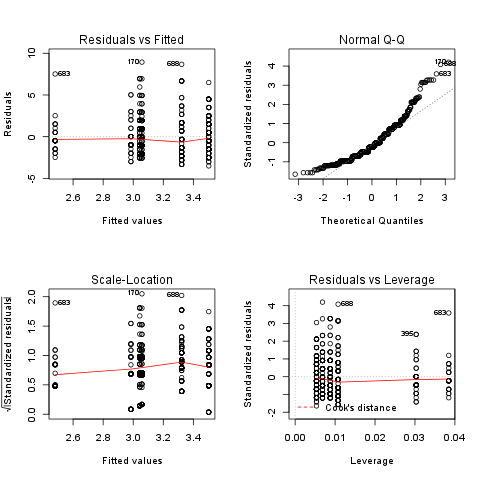
\includegraphics{efd197b02ca1541c48611907a3c42576.png}
\caption{}
\end{figure}

\subsection{ANOVA Summary}

\subsubsection{ANOVA Table}

\ctable[pos = H, center, botcap]{llllll}
{% notes
}
{% rows
\FL
 & \textbf{Df} & \textbf{Sum.Sq} & \textbf{Mean.Sq} & \textbf{F.value} & \textbf{Pr..F.}
\ML
gender & 1 & 4.9473 & 4.9473 & 1.0853 & 0.2979
\\\noalign{\medskip}
partner & 2 & 31.2124 & 15.6062 & 3.4237 & 0.0332
\\\noalign{\medskip}
gender:partner & 2 & 3.0375 & 1.5188 & 0.3332 & 0.7168
\\\noalign{\medskip}
Residuals & 593 & 2703.0899 & 4.5583 &  & 
\LL
}

\emph{F-test} for \emph{Gender} is not statistically significant, which
implies that there is no Gender effect on response variable. Effect of
\emph{Relationship status} on response variable is significant.
Interaction between levels of \emph{Gender} and \emph{Relationship
status} wasn't found significant (p = 0.717).

\begin{center}\rule{3in}{0.4pt}\end{center}

This report was generated with
\href{http://rapport-package.info/}{rapport}.

\begin{figure}[htbp]
\centering

\includegraphics{images/rapport.png}
\caption{}
\end{figure}

\end{document}
